\vspace{-1em}
\section{Results}
\label{sec:results}
\vspace{-1em}

We provide extensive simulation and experimental data and their interpretation,
supporting that the proposed analog signal generator works as intended.

\vspace{-1em}
\subsection{Simulation}
\vspace{-1em}

We perform a realistic LTSpice~\cite{ltspice} simulation of both second-order
filters derived in Sections~(\ref{ssec:second}, \ref{ssec:sallenkey}). One of
the important aspects of these designs is the selection of the op-amp. In order
to keep the common-mode voltage at $0$\unit{\volt} we choose the op-amps as CMOS
type. One such op-amp is \texttt{OP292}~\cite{op292}, which is used in this
simulation.

The PWM signal generated by Teensy~\cite{teensy} is simulated exactly with a
carrier frequency of $36.6$\unit{\kilo\hertz} modulating the signal \[
V_{\text{pwm}} = \nicefrac{3.3}{2} + \nicefrac{3.3}{2}\sin{(2\pi 90 t)}.\]
Finally, the impedance of the load (PI's controller) is read off from its
datasheet and inserted as a $100$\unit{\kilo\ohm} resistance. The circuit that
is simulated using LTSpice is presented in Figures~\ref{fig:real_sig_gen}
and~\ref{fig:sallenkey_sim} (the bottom plot).

\begin{figure}[htb] 
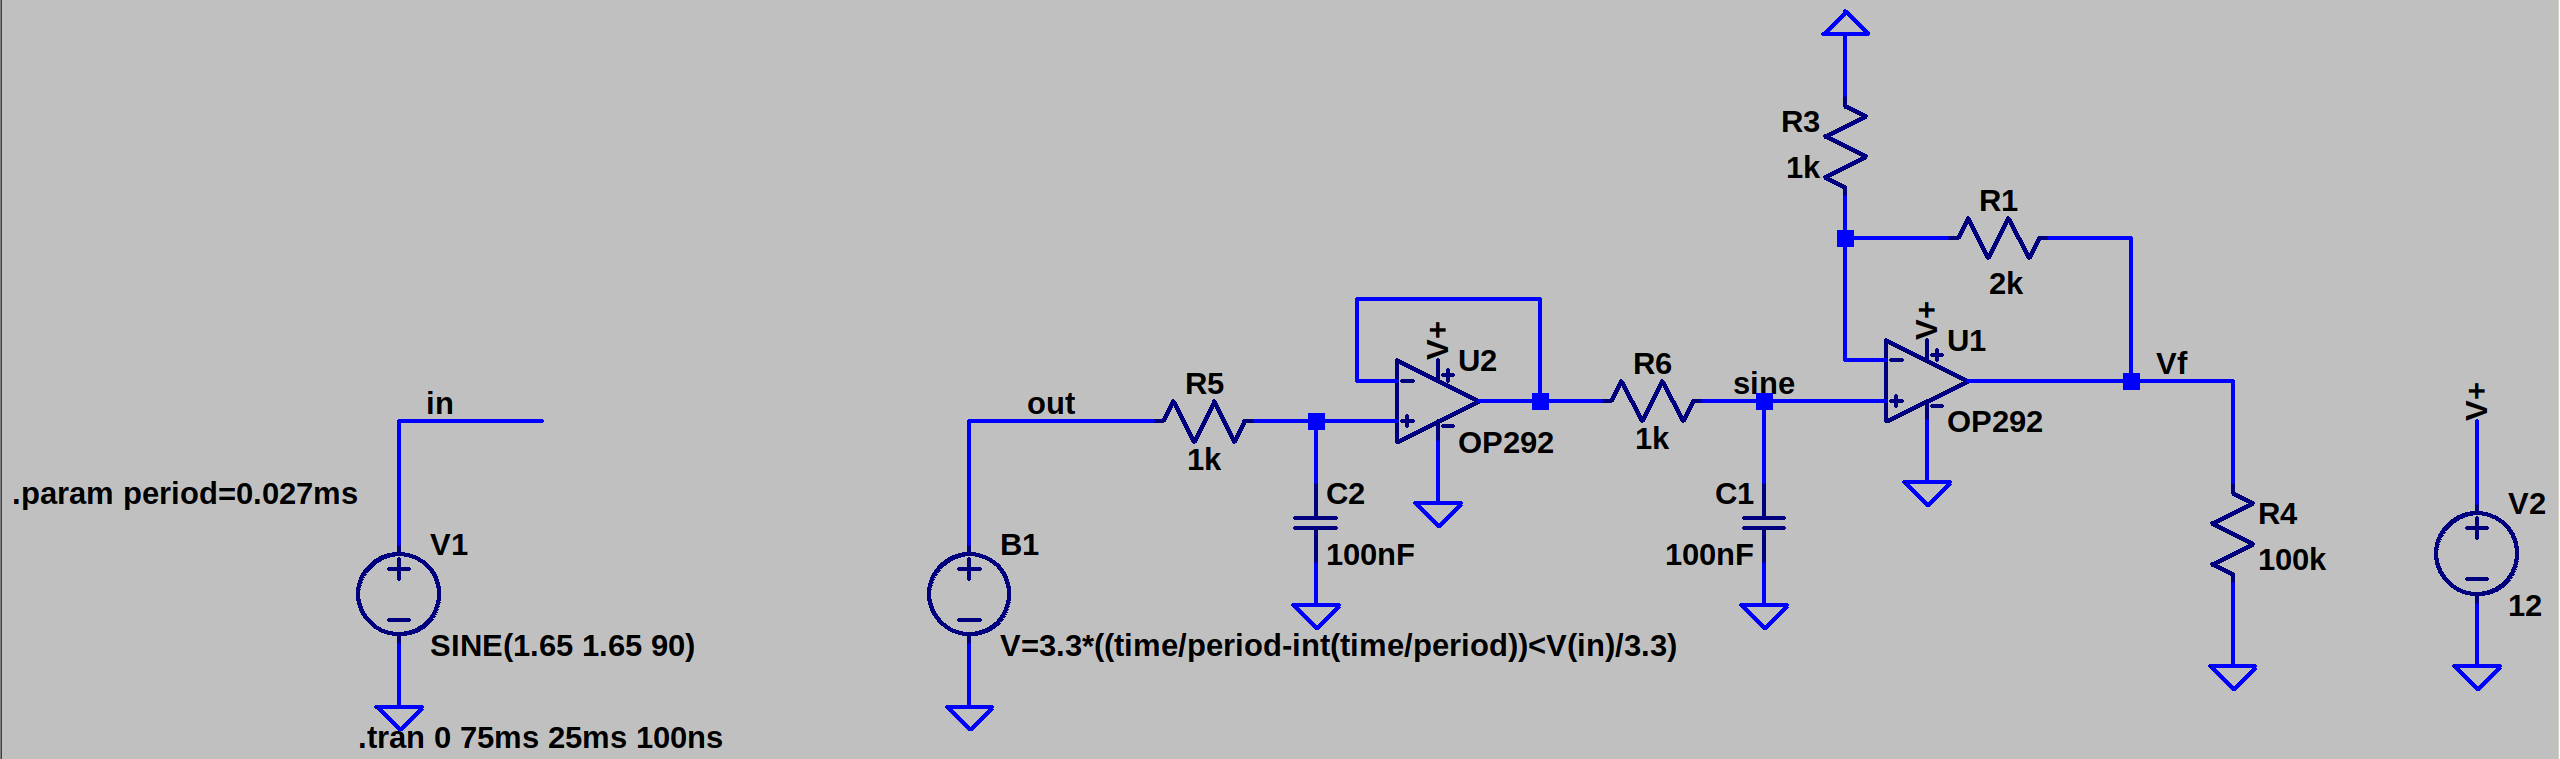
\includegraphics[width=8cm]{./figures/circuit.png}
\caption{The signal generator circuit in LTSpice} 
\label{fig:real_sig_gen}
\end{figure}

The simulation for the architecture in Section~\ref{ssec:second} generates the
relevant voltage responses, provided in Figure~\ref{fig:response}. The top plot
shows the PWM signal generated by Teensy modulating a sine-wave at
$90$\unit{\hertz} frequency. The individual plots in the middle show the output
of the first (cyan) and the second (purple) RC low-pass filters ($v_m$ and
$v_i$, respectivel) that extract the modulated signal from its PWM
representation. Finally, the last plot shows the thrice amplified signal through
the op-amp \texttt{OP292}.

\begin{figure}[t]
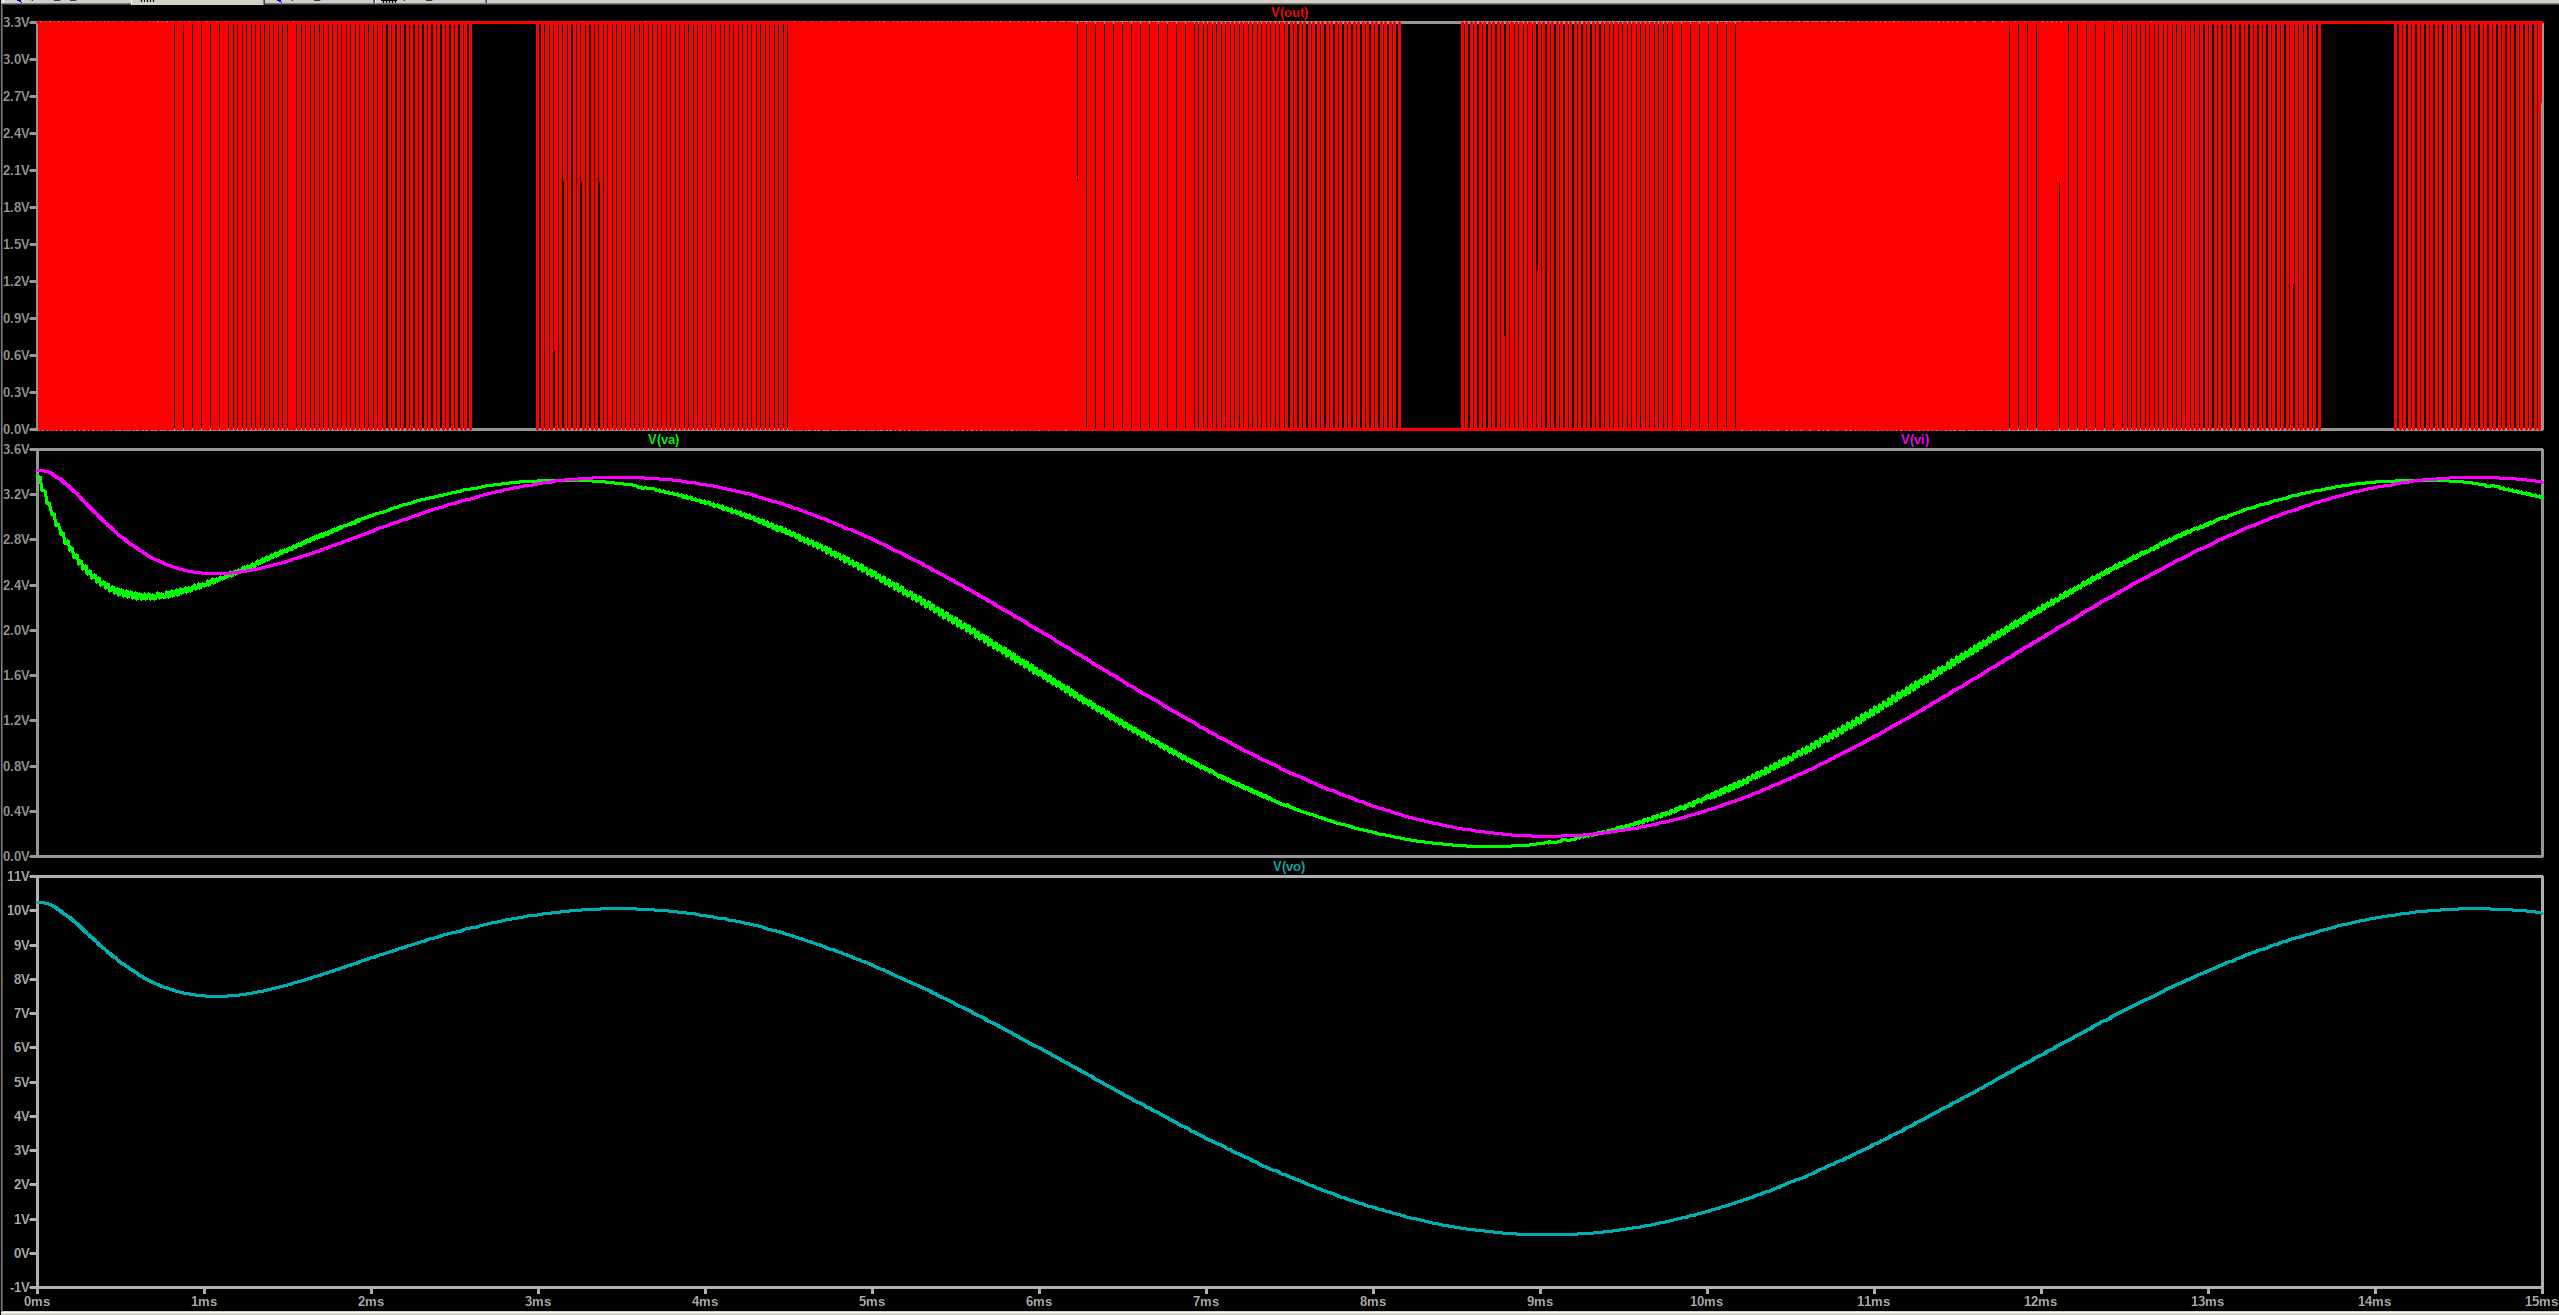
\includegraphics[width=0.5\textwidth]{./figures/pwm_filtered_one_two_final_signal.png}
\caption{The response from the simulation for one full period.} 
\label{fig:response}
\end{figure}


The performance of the Sallen-Key architecture from Section~\ref{ssec:sallenkey}
is shown in Figure~\ref{fig:sallenkey_sim} (top plot), where the values for the
resistances were taken to be $R_d = 68$\unit{\kilo\ohm} and capacitances to be
$C_d = 1$\unit{\nano\farad}. Even though the performance of the Sallen-Key
filter of Section~\ref{ssec:sallenkey} looks very similar to the $RC$+buffer
filter of Secton~\ref{ssec:second} in simulation, the experiments favor the
Sallen-Key significantly. We will implement this filter in our final design.

\begin{figure}[tbh]
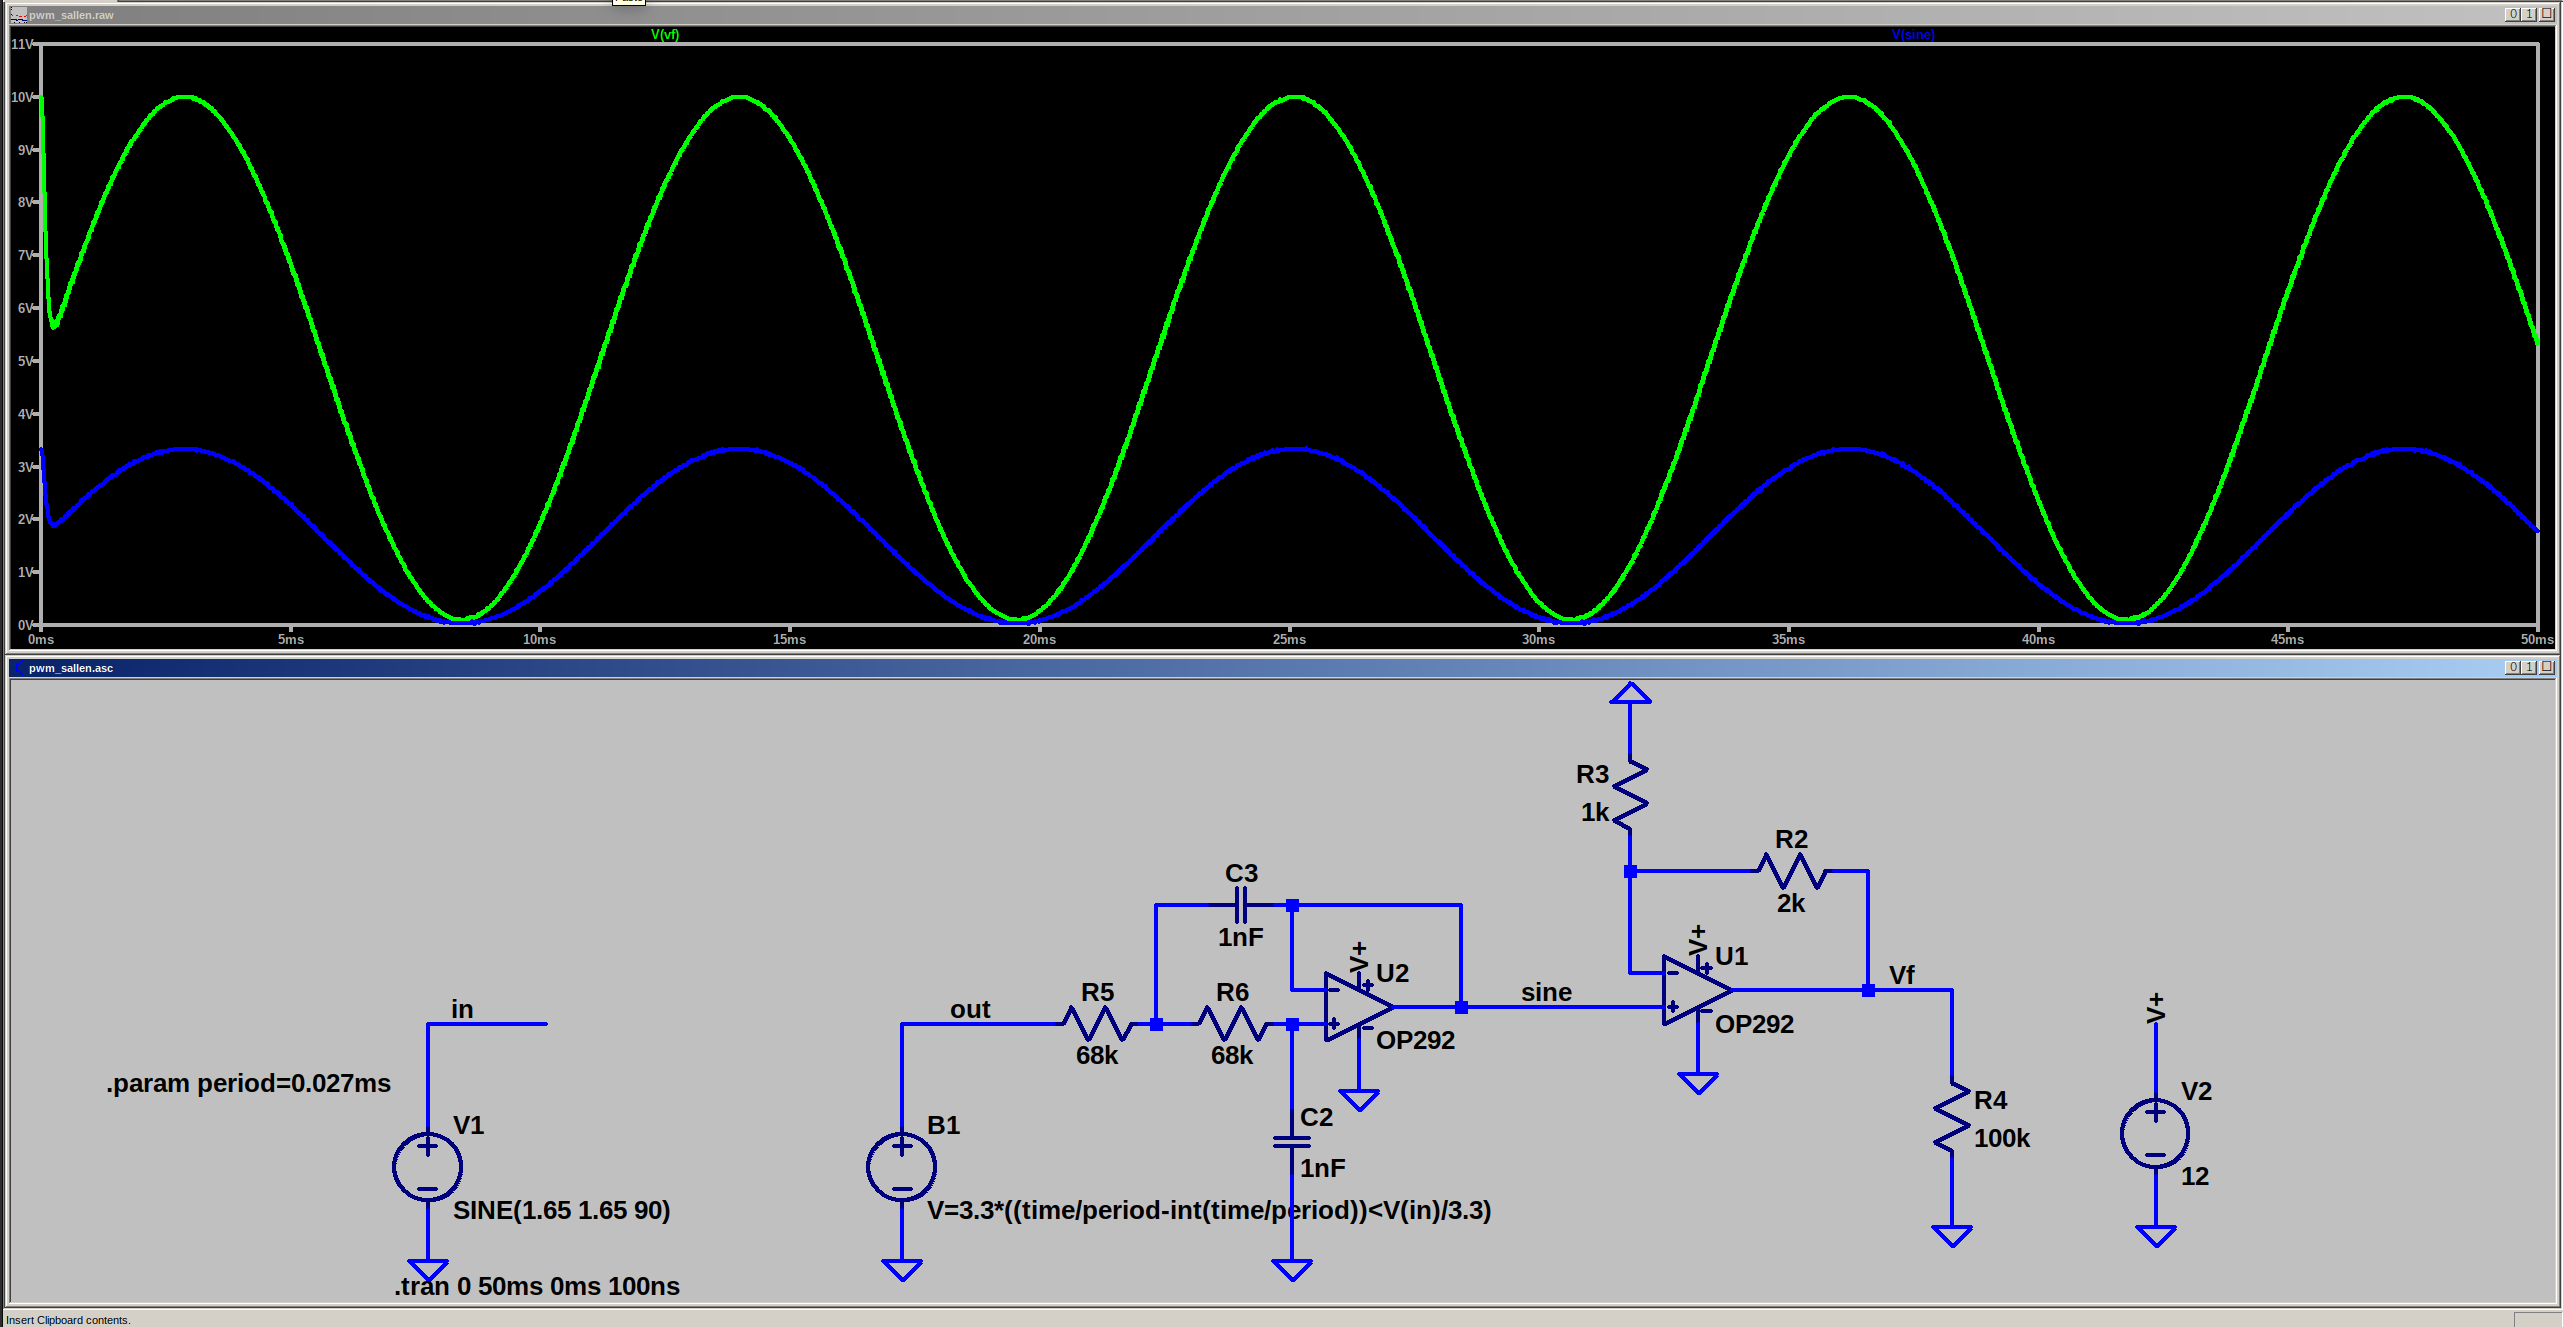
\includegraphics[width=0.5\textwidth]{./figures/sallenkey.png}
\caption{The response of the Sallen-Key architecture.}
\label{fig:sallenkey_sim}
\end{figure}


\vspace{-1em}
\subsection{Experiment}
\vspace{-1em}

The Sallen-Key architecture is implemented on a simple setup on my tabletop.

% \begin{figure}[t]
% 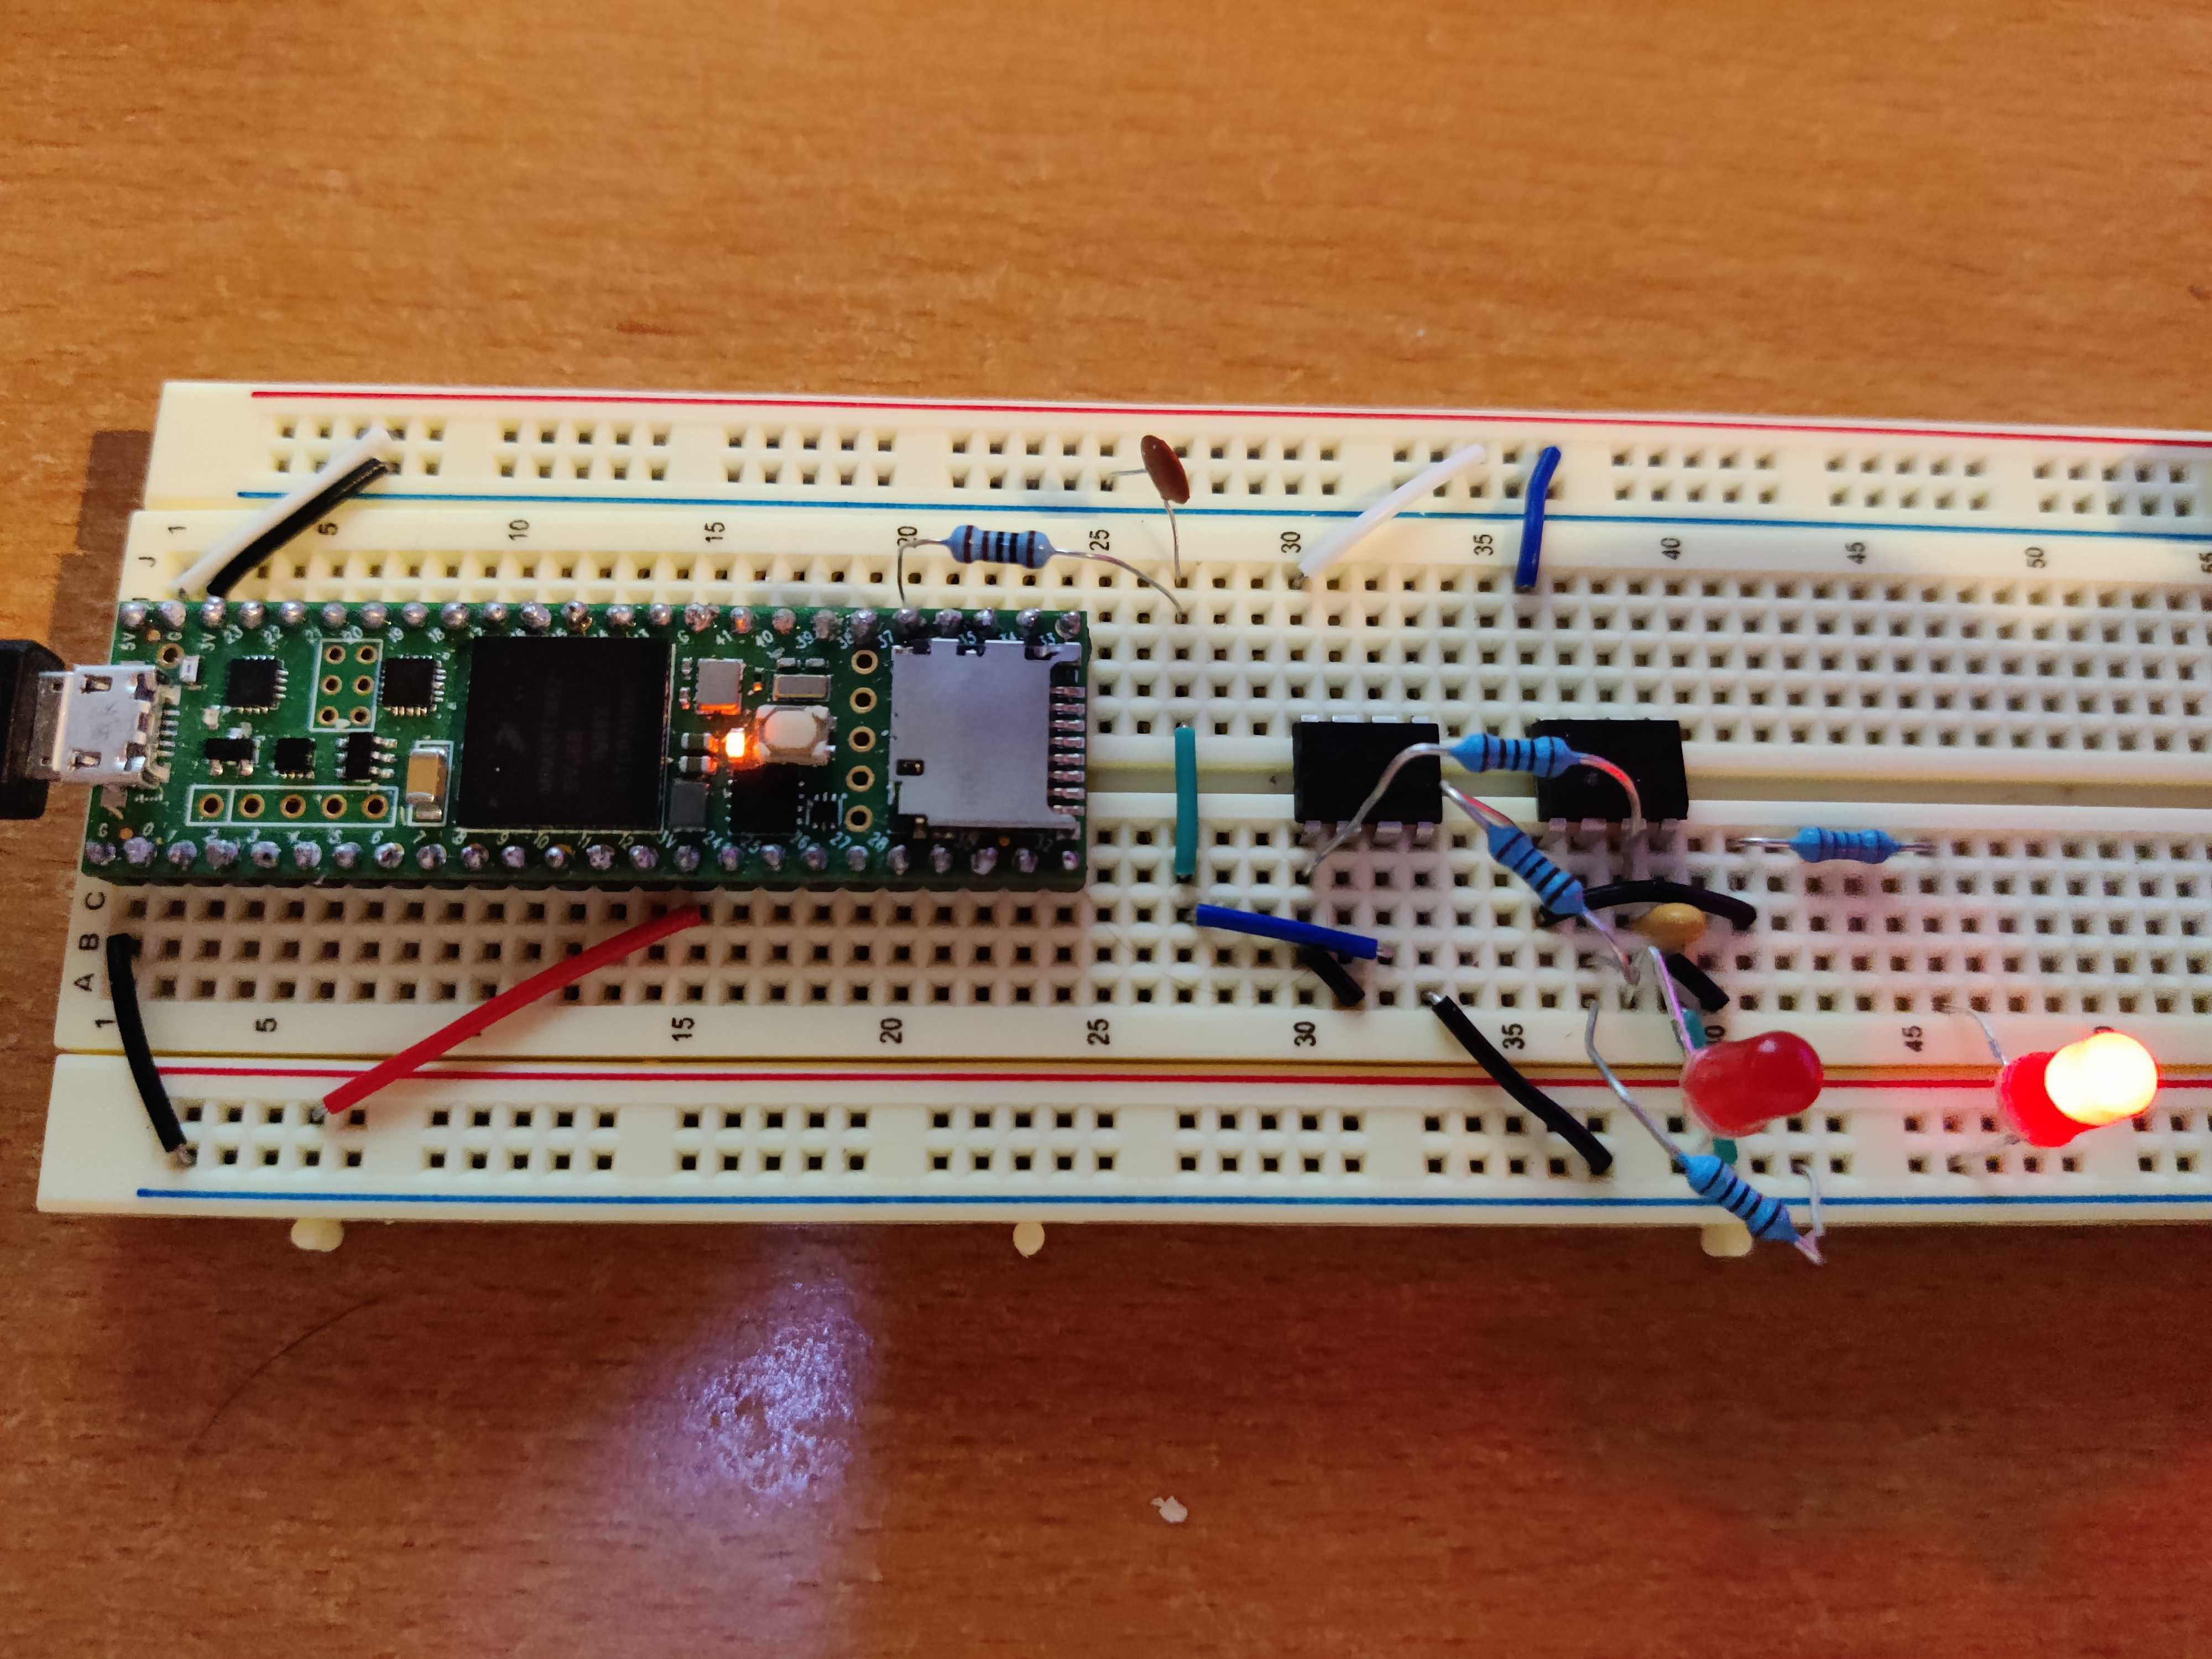
\includegraphics[width=0.5\textwidth]{./figures/prototype.jpg}
% \caption{Prototype working on a LED} 
% \label{fig:exp}
% \end{figure}

\begin{figure}[bh]
    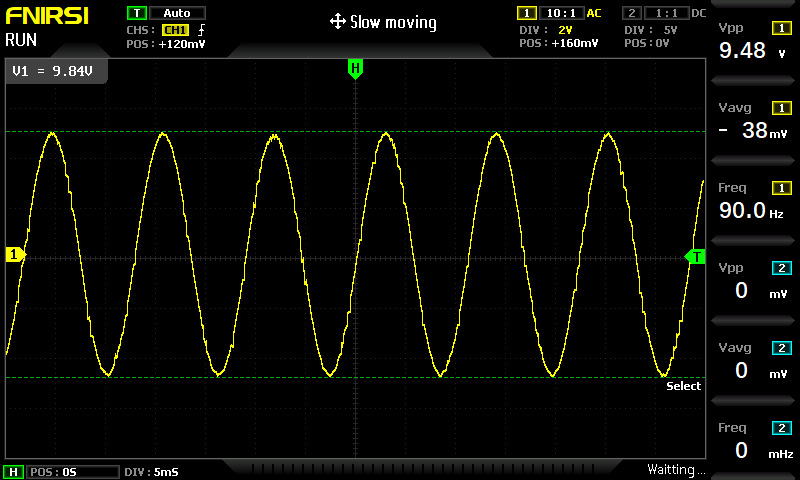
\includegraphics[width=0.5\textwidth]{./figures/output_osc.jpg}
    \caption{The response of the second-order Sallen-Key filter.}
    \label{fig:sallenkey_osc}
\end{figure}

Figure~\ref{fig:sallenkey_osc} shows the response of the second-order Sallen-Key
LPF observed through an oscilloscope. This is the output of the signal generator
in response to the Teensy generated $90$\unit{\hertz} $0-3.3$\unit{\volt} PWM
signal modulating the desired sine wave. This response is satisfactory and
should drive the PI controller without any issues.
